\documentclass[a4paper, magyar]{article}

\usepackage[utf8]{inputenc}
\usepackage[magyar, english]{babel}
\usepackage[T1]{fontenc}
\usepackage{testhyphens}
\usepackage{multirow}
\usepackage{graphicx}

%--------------------------------------------------------------------------------------
% Main variables
%--------------------------------------------------------------------------------------
\newcommand{\vikszerzo}{Németh Gergely Dániel}
\newcommand{\vikkonzulens}{Ács Judit}
\newcommand{\vikcim}{Deep Learning alapú szótagolás}
\newcommand{\viktanszek}{Automatizálási és Alkalmazott Informatikai Tanszék}
\newcommand{\vikdoktipus}{Önnáló laboratórium}

\newcommand{\secref}[1]{\aref{#1}.~fejezet}
\newcommand{\figref}[1]{\aref{#1}.~ábr}
\newcommand{\tabref}[1]{\aref{#1}.~táblázat}
\newcommand{\Secref}[1]{\Aref{#1}.~fejezet}
\newcommand{\Figref}[1]{\Aref{#1}.~ábr}
\newcommand{\Tabref}[1]{\Aref{#1}.~táblázat}
%--------------------------------------------------------------------------------------
%	The title page
%--------------------------------------------------------------------------------------
\begin{document}
\selectlanguage{magyar}

\begin{titlepage}
	\begin{center}
		
\includegraphics[width=60mm,keepaspectratio]{figures/BMElogo.png}\\
		\vspace{0.3cm}
		\textbf{Budapesti Műszaki és Gazdaságtudományi Egyetem}\\
		\textmd{Villamosmérnöki és Informatikai Kar}\\
		\textmd{\viktanszek}\\[5cm]
		
		\vspace{0.4cm}
		{\huge \bfseries \vikcim}\\[0.8cm]
		\vspace{0.5cm}
		\textsc{\Large \vikdoktipus}\\[4cm]
		
		\begin{tabular}{cc}
			\makebox[5.5cm]{\emph{Készítette}} & \makebox[5.5cm]{\emph{Konzulens}} \\
			\makebox[5.5cm]{\vikszerzo} & \makebox[5.5cm]{\vikkonzulens}
		\end{tabular}
		
		\vfill
		{\large \today}
	\end{center}
\end{titlepage}


%---

	
\fontfamily{ptm}\selectfont

\selectlanguage{english}
\begin{abstract}

\end{abstract}
\vfill
\selectlanguage{magyar}
\begin{abstract}
	
\end{abstract}
\vfill
\newpage
\tableofcontents
\newpage
\section{Bevezetés}
\section{Szótagoló programok}
Az elterjedt szótagoló algoritmusok kétféle csoportba bonthatóak: szabály- vagy szótáralapúak. A szabad szoftverek világában \textit{de facto} a \TeX szótagolási algoritmusát használják.

A \TeX\,eredeti szótagoló algoritmusát Prof. Knuth tervezte 1977 nyarán \cite{knuth1979tex}. Ez három fő szótagolási szabályt alkalmazott: $1)$ utótag leválasztás, $2)$ előtag leválasztás és $3)$ magánhangzó - mássalhangzó - mássalhangzó - magánhangzó (vccv) elválasztás, azaz ha ilyen betűnégyes található a szóban, legtöbb esetben a mássalhangzók mentén elválasztható. Ez a három szabály gyakran alkalmazható, azonban már az első algoritmusban kiegészült kisebb szabályokkal (,,break vowel-q" vagy ,,break after ck") és kivételek listájával(300 szó).

A \TeX82 verzióhoz megjelent Liang szótagoló algoritmusa \cite{liang1983word}, aminek legfontosabb újítása a minta(\textit{patterns}) alapú szótagolás bevezetése volt. Ennek lényege, hogy a szótagolási szabályok mintákra definiálódtak és az algoritmus a szótagolás során ezeket a mintákat keresi a szóban.

A \TeX\,jelenlegi verziójában a Hunspell szótagoló algoritmust alkalmazzák \cite{nemeth2006automatic}. Ez az eljárás Liang algoritmusán alapszik, amit nyelvfüggő speciális szótagolási kiterjesztésekkel (\textit{non-standard hyphenation extension}) egészít ki.
\subsection{Liang algoritmusa}
Liang szótagoló algoritmusának alapját a szótagolási minták alkotják \cite{liang1983word}. Az algoritmust az angol 
{\fontfamily{pcr}\selectfont
	hyphenation%
} elválasztását az alábbi módon végzi:

Az algoritmus először megnézi, hogy a szó benne van-e a kivételek listájában (ez lényegében teljes szavakat tartalmaz mintaként). A \textit{hyphenation} szó nincs a kivételek listájában.

Ezután a szó elejére és végére illeszt egy pont  jelző karaktert. Ennek jelentősége azoknál a mintáknál lesz, amelyek akkor érvényesülnek, ha a szó elején, vagy a végén szerepelnek.
{\fontfamily{pcr}\selectfont
	\begin{center}
	.hyphenation.
	\end{center}
}
Ezt követően a minták között keres illeszkedést. A \textit{hyphenation} szóra ezek az alábbiak: 
{\fontfamily{pcr}\selectfont hy3ph, he2n, hena4, hen5at, 1na, n2at, 1tio,  2io}  \cite[37.\ oldal]{liang1983word}
A megfelelő mintákat ráillesztve a szóra, a bennük szereplő számokat a szó karakterei közé szúrva az \ref{liang-hyp}. ábrán szereplőket kapjuk.%
\footnote{Az ábrázolásmód N{\'e}meth cikkéből származik \cite{nemeth2006automatic}.}
\begin{figure}[ht]\centering
	{\fontfamily{pcr}\selectfont
		\setlength{\tabcolsep}{0pt}
		\begin{tabular}{rrrrrrrrrrrrr}
			.& h& y& p& h& e& n& a & t& i& o& n& .\\
			 & h& y&3p& h\\
			 &  &  &  & h& e&2n\\
			 &  &  &  & h& e& n& a&4\phantom{t}\\
			 &  &  &  & h& e& n&5a&t\\
			 &  &  &  &  &  &1n& a\\
			 &  &  &  &  &  & n&2a& t\\
			 &  &  &  &  &  &  &  &1t& i& o\\
			 &  &  &  &  &  &  &  &  &2i& o\\
			 \hline
			 .&0h&0y&3p&0h&0e&2n&5a&4t&2i&0o&0n&0.\\
			  & h& y&-p& h& e& n&-a& t& i& o& n
		\end{tabular}
	}
\caption{A \textit{hyphenation} szótagolása}\par\medskip\centering
\label{liang-hyp}
\end{figure}


Az algoritmus következő lépésében minden két szomszédos karakter közé illesztünk egy számot. Alapértelmezetten $0$-t és ha ennél nagyobb számot találtunk a mintaillesztésnél, a legnagyobb kapott értéket adjuk meg.

A szótagolás szabálya innen már csak egy lépés: a páratlan számok mentén elválasztunk, a párosoknál nem. Ezzel megkaptuk a
{\fontfamily{pcr}\selectfont
	hy-phen-ation%
}
elválasztást.
\subsubsection{Minták választása}
A fenti algoritmus hatékonyságát nyilvánvalóan a minták mennyisége és hatékonysága határozza meg. Csak azok a szavak választódnak el, amelyekre illeszkedik minta és csak azok lesznek jó elválasztások, melyekre jó minta illeszkedik.

\subsection{Hunspell}
\subsubsection{Szótagolási hibák a magyar Hunspellben}


\begin{minipage}{0.5\textwidth}
	Hunspell szótagolása:
\begin{checkhyphens}
	autóval
	
	szemüveggel
	
	hasizom
	
	messze
\end{checkhyphens} 		
\end{minipage}\noindent
\begin{minipage}{0.5\textwidth}
	Helyesen:

	a-u-tó-val\\
	szem-ü-veg-gel\\
	has-i-zom\\
	mesz-sze
\end{minipage}


\section{Deep learning alapú módszerek}
\subsection{Deep learning bevezetés}
A gépi tanulás területén egyre nagyobb teret nyernek a deep learning alapú módszerek. A hagyományos osztályozási feladatokon túl, szekvenciális, ún. taggelési problémák megoldására is alkalmasak a neurális hálók, különös tekintettel a rekurrens neurális hálókra.

A mély tanulás bevetését a nyelvtechnológia területén az a tény élteti, hogy az elektronikus kommunikáció korában jelentős mennyiségű nyelvi adatbázisok állnak rendelkezésünkre, így a deep learning legfontosabb eleme, a megfelelő méretű tanulóadat elérhető. Az ismertetett elválasztási algoritmusok kulcseleme, hogy megfelelő elválasztási mintákat ismerjünk fel az adathalmazon (\textit{korpusz}). A képfelismerés terén sokkal komplexebb minták megtalálásában is jelentős eredményeket értek el a deep learning segítségével, így e módszer bevetése a szótagolás problémakörében megalapozott.

\subsubsection{Keretrendszerek}
Deep learning rendszerek tervezésénél az utóbbi időben ipari és kutatói területen egyaránt elterjedőben vannak a magas szintű keretrendszerek. Ezek legnagyobb előnye, hogy az aktív fejlesztői közösség a gyorsan fejlődő tudományág eredményeit alkalmazható technológiákként tárja a felhasználók elé. A jelentősebb keretrendszerek: TensorFlow\footnote{TensorFlow: https://www.tensorflow.org/}, Torch7\footnote{Torch7: http://torch.ch/}, Keras\footnote{Keras: https://keras.io/}. Az itt ismertetett eljárások megvalósításához a Keras nyújtotta lehetőségekkel valósultak meg \cite{chollet2015keras}.
\subsection{Tanító adatok}
Mély tanulás esetén az eredmény minőségét alapvetően meghatározza a tanítóhalmaz minősége. Jelen esetben a korpuszok és azok megfelelő szótagoltsága.

A hálótervezés során a Magyar Webkorpusz leggyakoribb $100000$ szaván kísérleteztünk \cite{halacsy2004creating,kornai2006web}.

\section{A feldolgozás folyamata}
A szótagoló jelenleg magyar nyelvre van tervezve, azonban az eljárás lényege univerzális.
\begin{figure}[htp]
	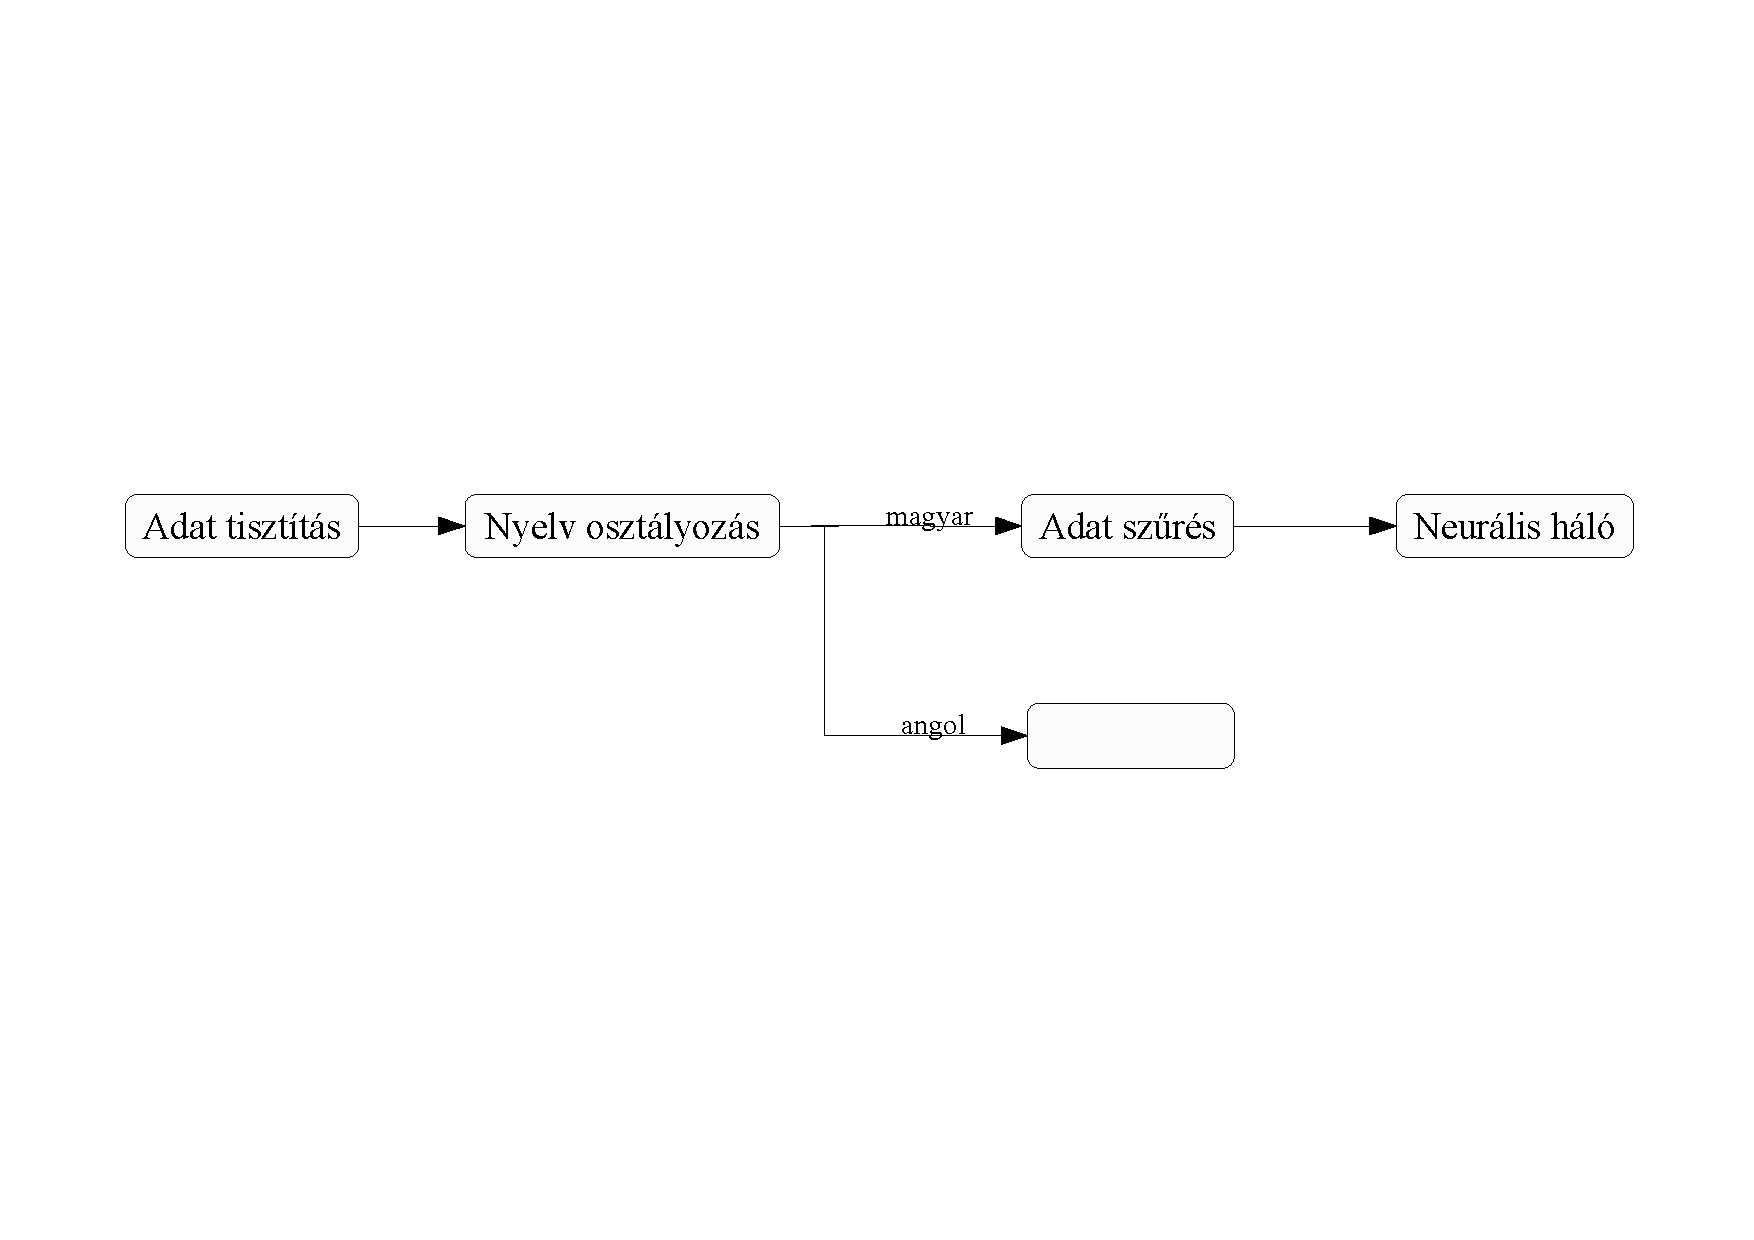
\includegraphics[trim={0 7cm 0 7cm},clip,
	width=\textwidth]{figures/preprocessing.pdf}
	\caption{A feldolgozás folyamata}\par\medskip\centering
	\label{fig:gui}
\end{figure}
\subsection{Adattisztítás}
Az adatfeldolgozás során az alábbi tisztítási eljárásokat végeztem:
\begin{description}
	\item[kisbetűsítés] A karaktereket kisbetűssé tettem.
	\item[speciális karakter szűrés] Az alábbi speciális karaktereket töröltem a szövegből(a \textit{python} {\fontfamily{pcr}\selectfont
		string.punctuation%
	} környezetfüggően választja meg ezeket, így máshol eltérhetnek): ! " \# \$ \% \& ' ( ) * + , - . / : ; < = > ? @ [ \\ ] \^{} \_ ` \{ | \} \~{}
	\item[szám szűrés] A szövegben található számokat töröltem.
\end{description}

Majd a szavakat egyedivé tettem (egy számlálóban eltárolva az előfordulási gyakoriságot).
\subsection{Adat szűrés}
A háló sajnos nem minden előforduló esetet tud kezelni, így a későbbi implementálásig ezeket szűröm.

\textbf{Speciális karakterek:} az adott nyelvre nem jellemző karakterek bezavarhatnak a tanításba, így ezeket célszerű kivenni. A magyar elválasztó esetén csak a magyar ábécé betűit hagytam meg.

\textbf{Kettős betűk:} az osztályozó jellegéből adódóan a plusz karakter bevonásával képződő elválasztást (például a \textit{ssz}-ből \textit{sz-sz}) a hálón kívül dolgozom fel.
\subsection{Nyelv osztályozó}
A tanítások kiértékelése során arra a következtetésre jutottam, hogy a hunspell és az én elválasztóm közötti eltérések jelentős része akkor adódik, ha idegen nyelvű szót próbálunk meg elválasztani. Így az elválasztó javításának érdekében egy nyelv osztályozót is bevezettem.

A jelenlegi nyelvválasztó egy egyszerű bigram gyakoriság alapú osztályozó.
%TODO
\section{Előrecsatolt neurális háló}
A neurális háló lényege ebben ez esetben az, hogy a szó minden karakterére eldöntsük a környezetében lévő karakterek segítségével, hogy a karakternél van-e elválasztás.

A szavakat minden karakter mentén felbontjuk az adott ablakméretre, majd ezekre az ablakokra tanítva oldunk meg egy osztályozó problémát, ami ad egy címkét a karakternek és a címke alapján végezzük az elválasztást.
\subsection{Karakter címkézés}
Kétféle címkézést használunk. Az első eset előnye, hogy több címke van így több információt adunk át a modellnek, a másodiké pedig, hogy a jósolt címkézés minden esetben elválasztássá alakítható. Ez a BMES esetében nem teljesül: ha két karakterre egymás után E-t jósol, az nem alakítható rögtön valós elválasztássá.

A jelenlegi munkában a BM címkézést elemeztük.
\paragraph{BMES}
\begin{itemize}
	\item B: Begin, szótag elején álló karakter
	\item M: Middle, közepén lévő karakter, se előtte, se utána nincs elválasztás
	\item E: End, a karakter után elválasztás van
	\item S: Single, egy karakterből álló szótag
\end{itemize}
A
{\fontfamily{pcr}\selectfont
	le-o-párd%
}
szó címkézése:
{\fontfamily{pcr}\selectfont
	BESBMME%
}
\paragraph{BM}
\begin{itemize}
	\item B: Begin, szótag elején álló karakter
	\item M: Minden egyéb eset
\end{itemize}
A
{\fontfamily{pcr}\selectfont
	le-o-párd%
}
szó címkézése:
{\fontfamily{pcr}\selectfont
	BMBBMMM%
}
\subsection{Adat-előkészítés}
\begin{figure}[htp]
	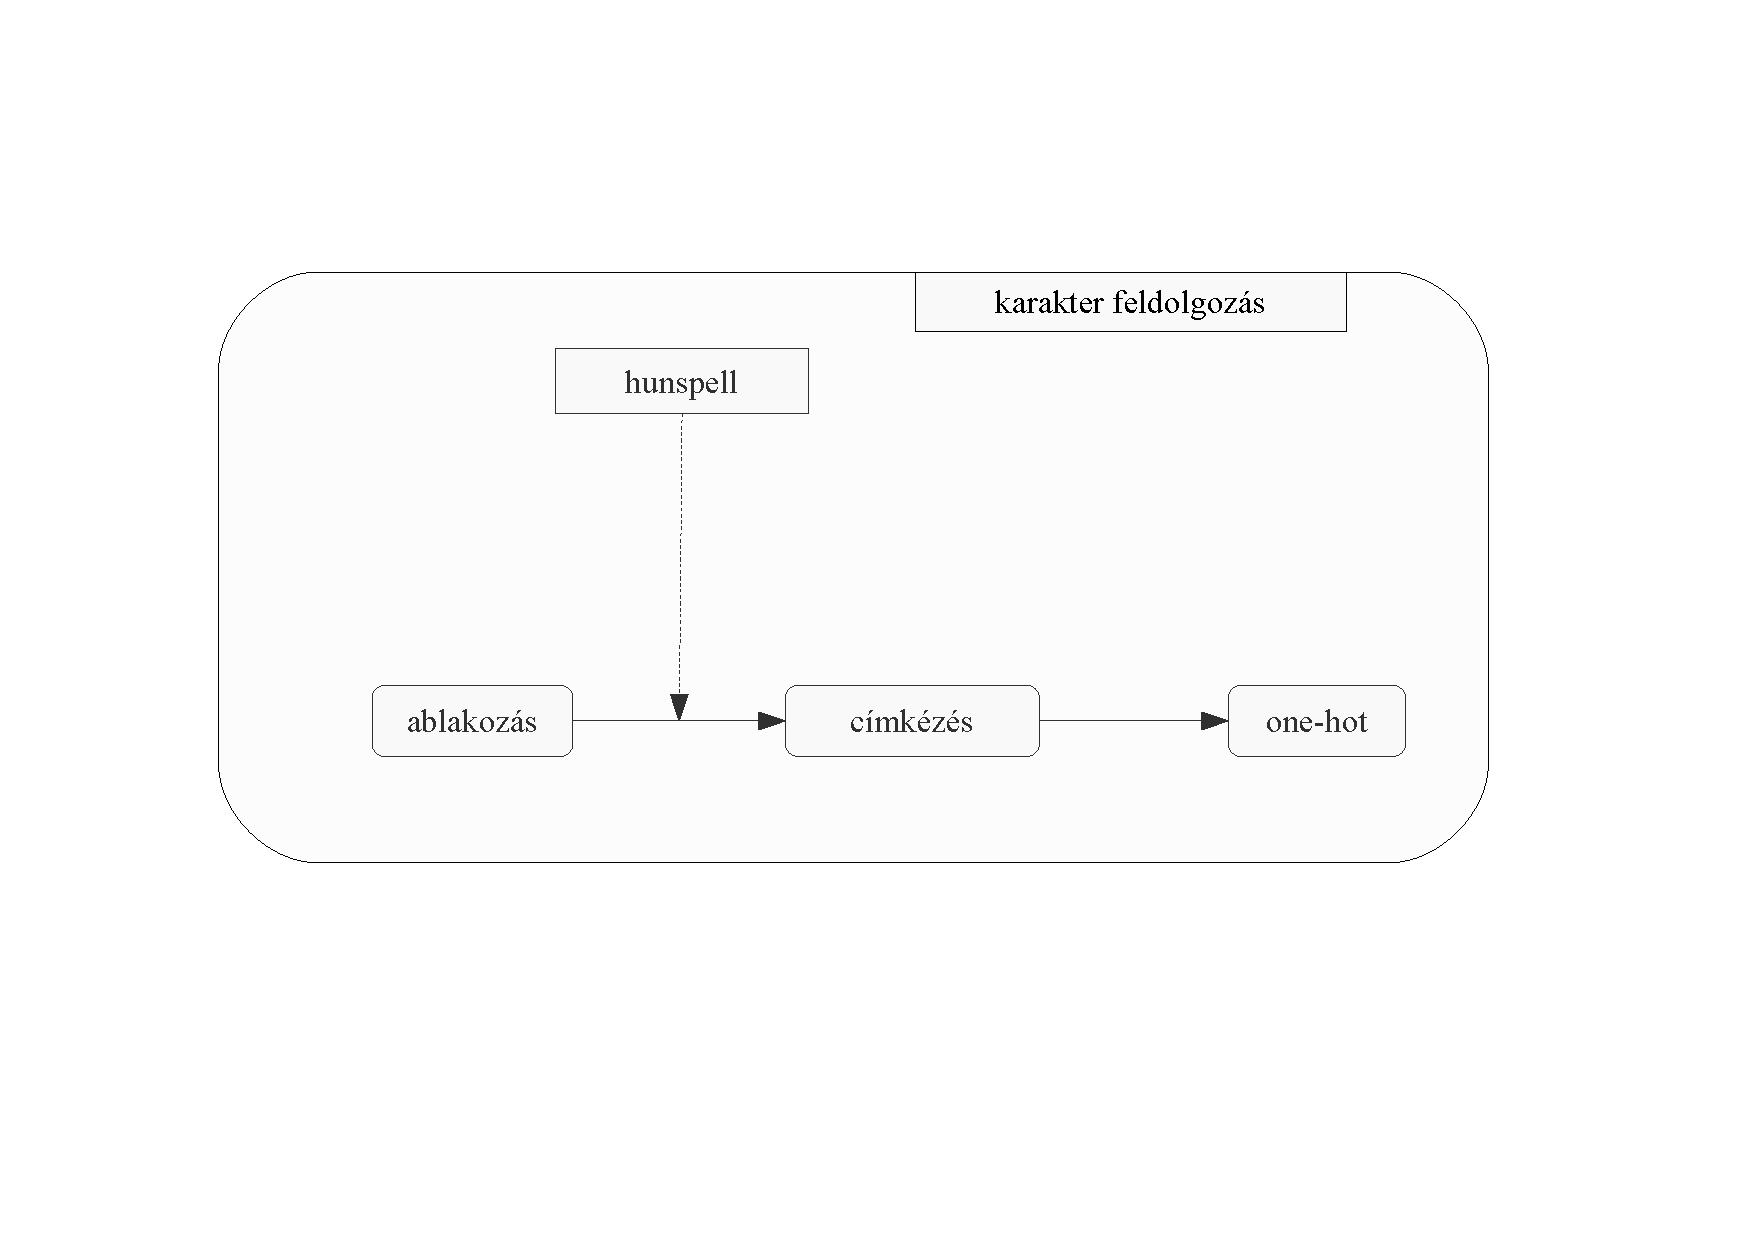
\includegraphics[trim={0 6cm 0 4cm},clip,
	width=\textwidth]{figures/characters.pdf}
	\caption{Tanítóadat előállítása}\par\medskip\centering
	\label{fig:char}
\end{figure}
Ha az \textit{nyúlanyó} szó \textit{a} karakterét szeretnénk egy $5$-ös szimmetrikus ablakú környezetben tanítóadatnak előkészíteni, \textbf{BM} címkézéssel, akkor az alábbi előkészületeket kell tennünk:
\subsubsection{Tanítás a karakter környezetéből}

A jelölésrendszerünk alapján az $5$-ös szimmetrikus ablak azt jelenti, hogy a karakter előtt és a karakter után is két-két további karaktert veszünk, és ez alapján az öt karakter alapján próbáljuk meg eldönteni, milyen címke illeszkedik a középső karakterre. Ezt jelöljük \textit{2-1-2}-vel. Az \textit{nyúlanyó} szó és az \textit{a} betű esetén ez \textit{úl\,a\,ny} ablakot jelent.

Ha az ablak túlnyúl a szó szélén, az elterjedt jelölés alapján a szó elején \^\ karaktereket, illetve a szó végén további \$ karaktereket illesztünk az ablakba.
\subsubsection{One-hot kódolás}

Ahhoz, hogy a karakterekből a keras által feldolgozható tanítóadat legyen, one-hot kódolást végzünk rajta. 

A karakterek esetében ez azt jelenti, hogy a megengedett karaktereket, jelen esetben a magyar ábécé karaktereit és a kezdő-, befejezőkaraktereket egymás után felsoroljuk, majd az adott karaktert úgy reprezentáljuk, hogy egy ezzel azonos hosszúságú tömbben a karakternek megfelelő sorszámú helyre egyest, minden további mezőbe nullást írunk.

A \textbf{BM} illetve \textbf{BMES} címkézést ugyanígy reprezentáljuk egy $2$ avagy $4$ hosszú tömbbel. 

\subsubsection{Lapítás}

Ha a fentieket elvégezzük egy $5$ hosszú ablakra, akkor a magyar ábécét figyelembe véve $5$ darab $35+2$ hosszú tömböt kapunk. A háló bemenetét úgy kapjuk meg, hogy ezt ellapítjuk egy $5\cdot37$ hosszú tömbbé (amiben $5$ helyen $1$-es, minden további helyen $0$-ás szerepel). Ez lesz a tanítóadatunk.
\subsection{Tanító-, validációs- és tesztadatok}
\begin{figure}[htp]
	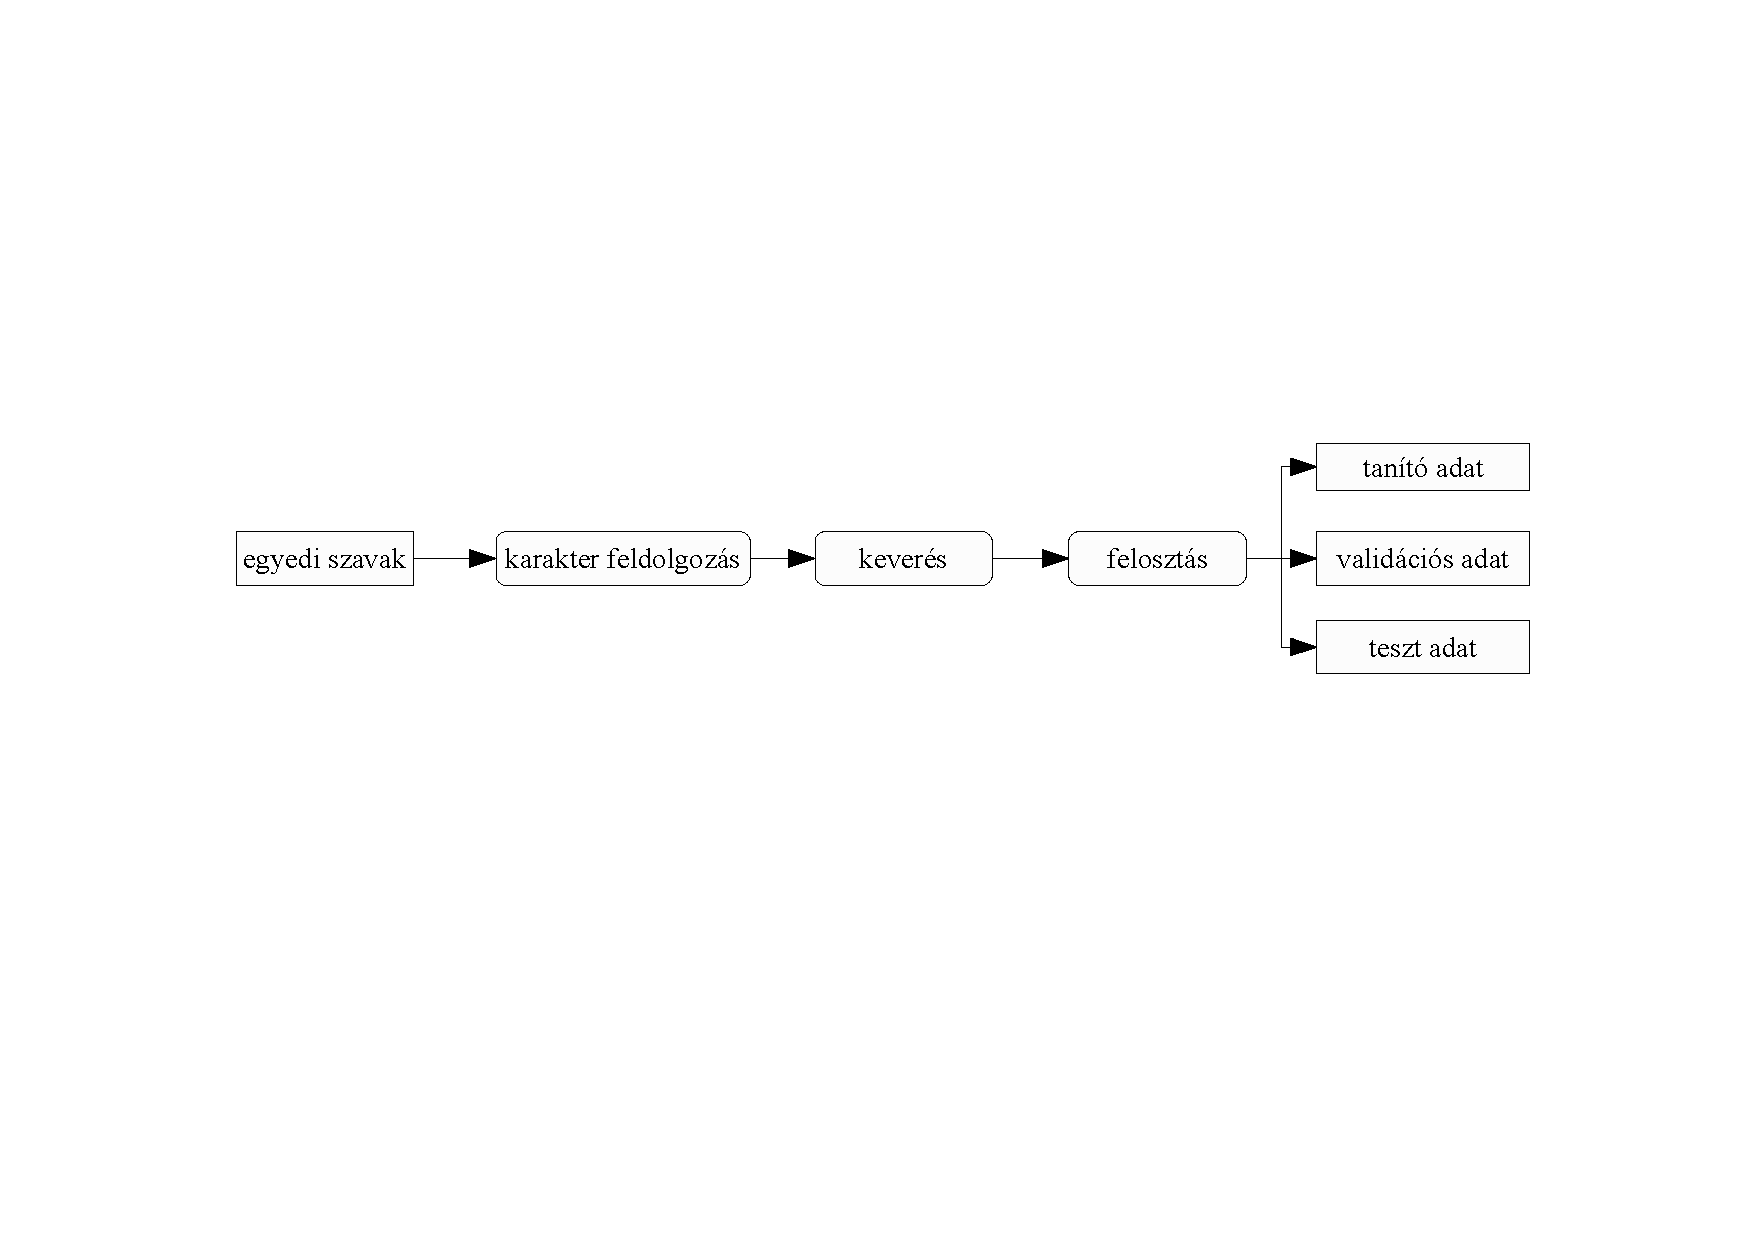
\includegraphics[trim={0 9cm 0 7cm},clip,
	width=\textwidth]{figures/dataflowdefault.pdf}
	\caption{A kezdeti adatgenerálás}\par\medskip\centering
	\label{fig:dfdef}
\end{figure}
\begin{figure}[htp]
	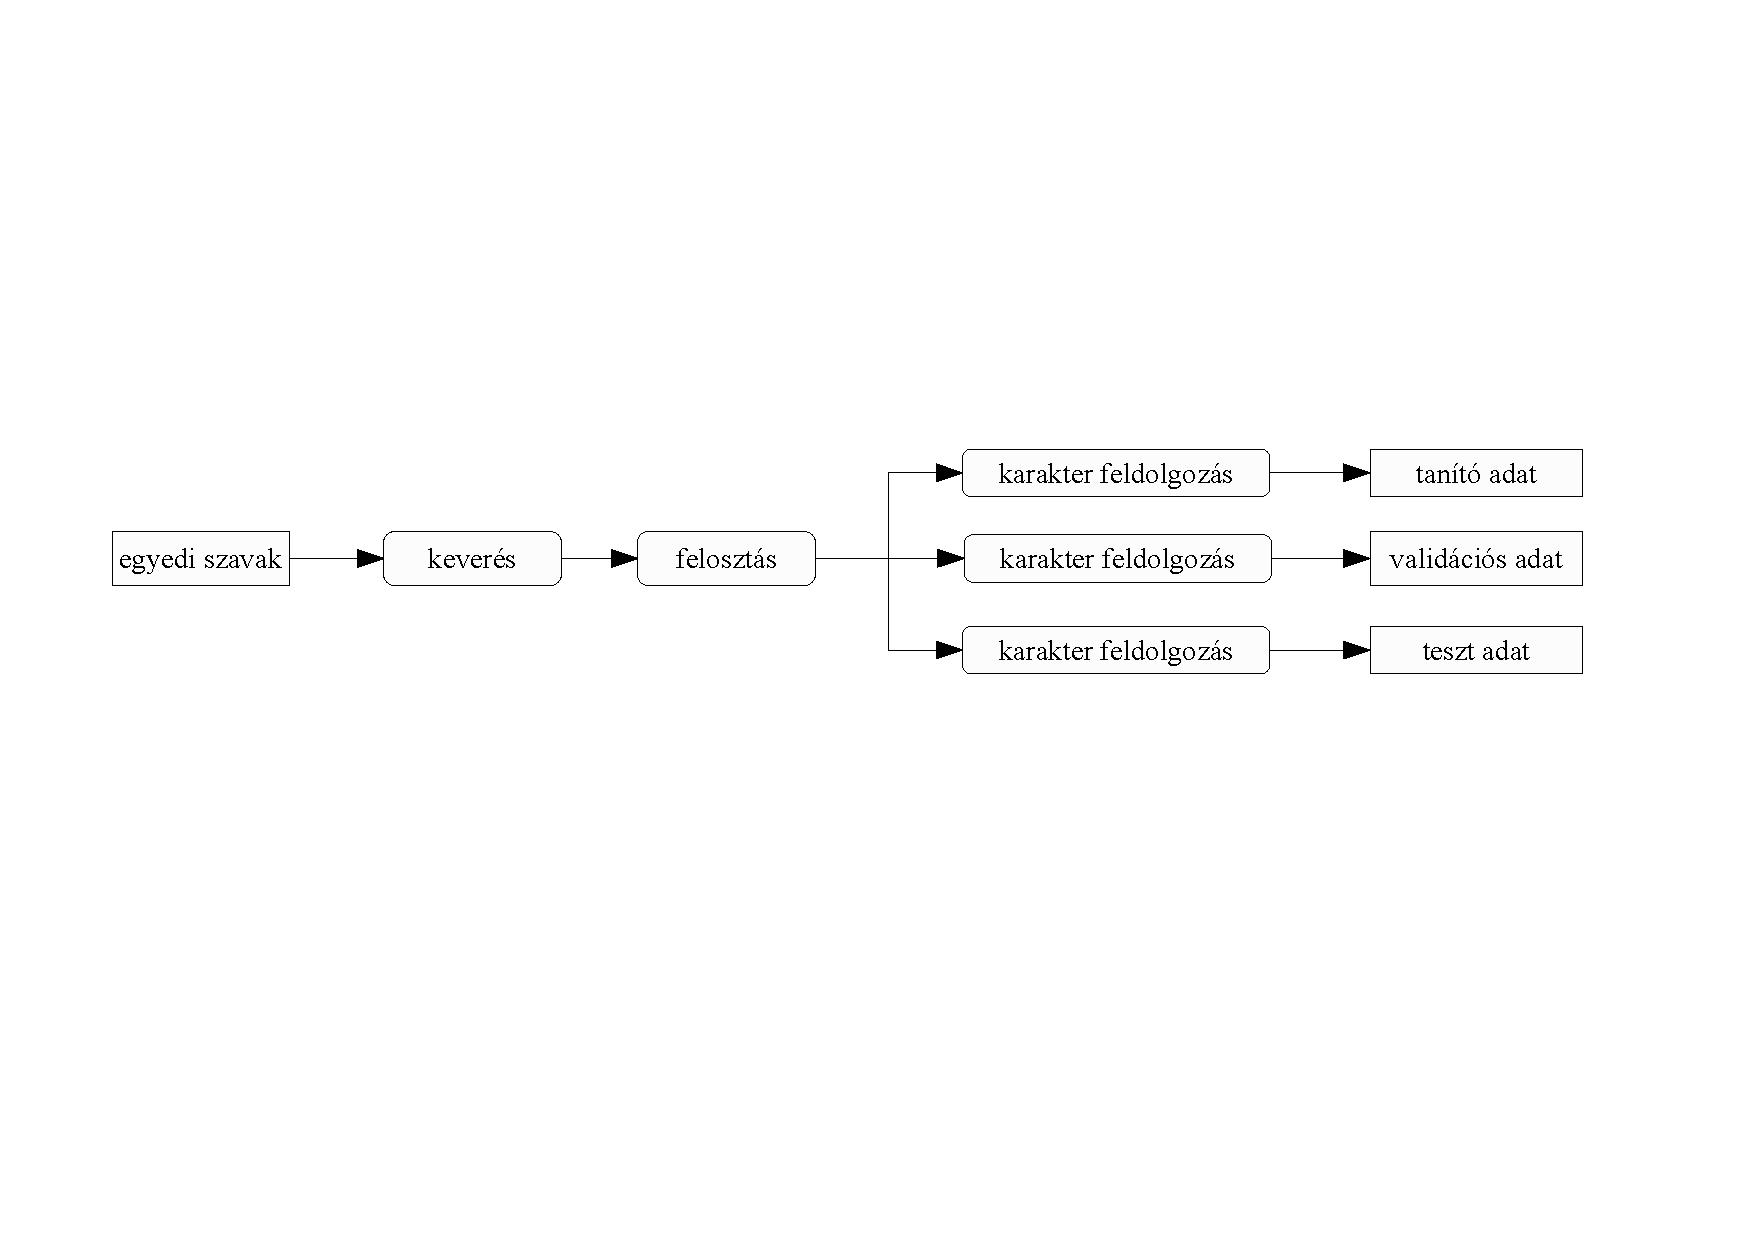
\includegraphics[trim={0 8cm 0 7cm},clip,
	width=\textwidth]{figures/dataflowuwords.pdf}
	\caption{Egyedi szavak felosztása}\par\medskip\centering
	\label{fig:dfuwords}
\end{figure}
\begin{figure}[htp]
	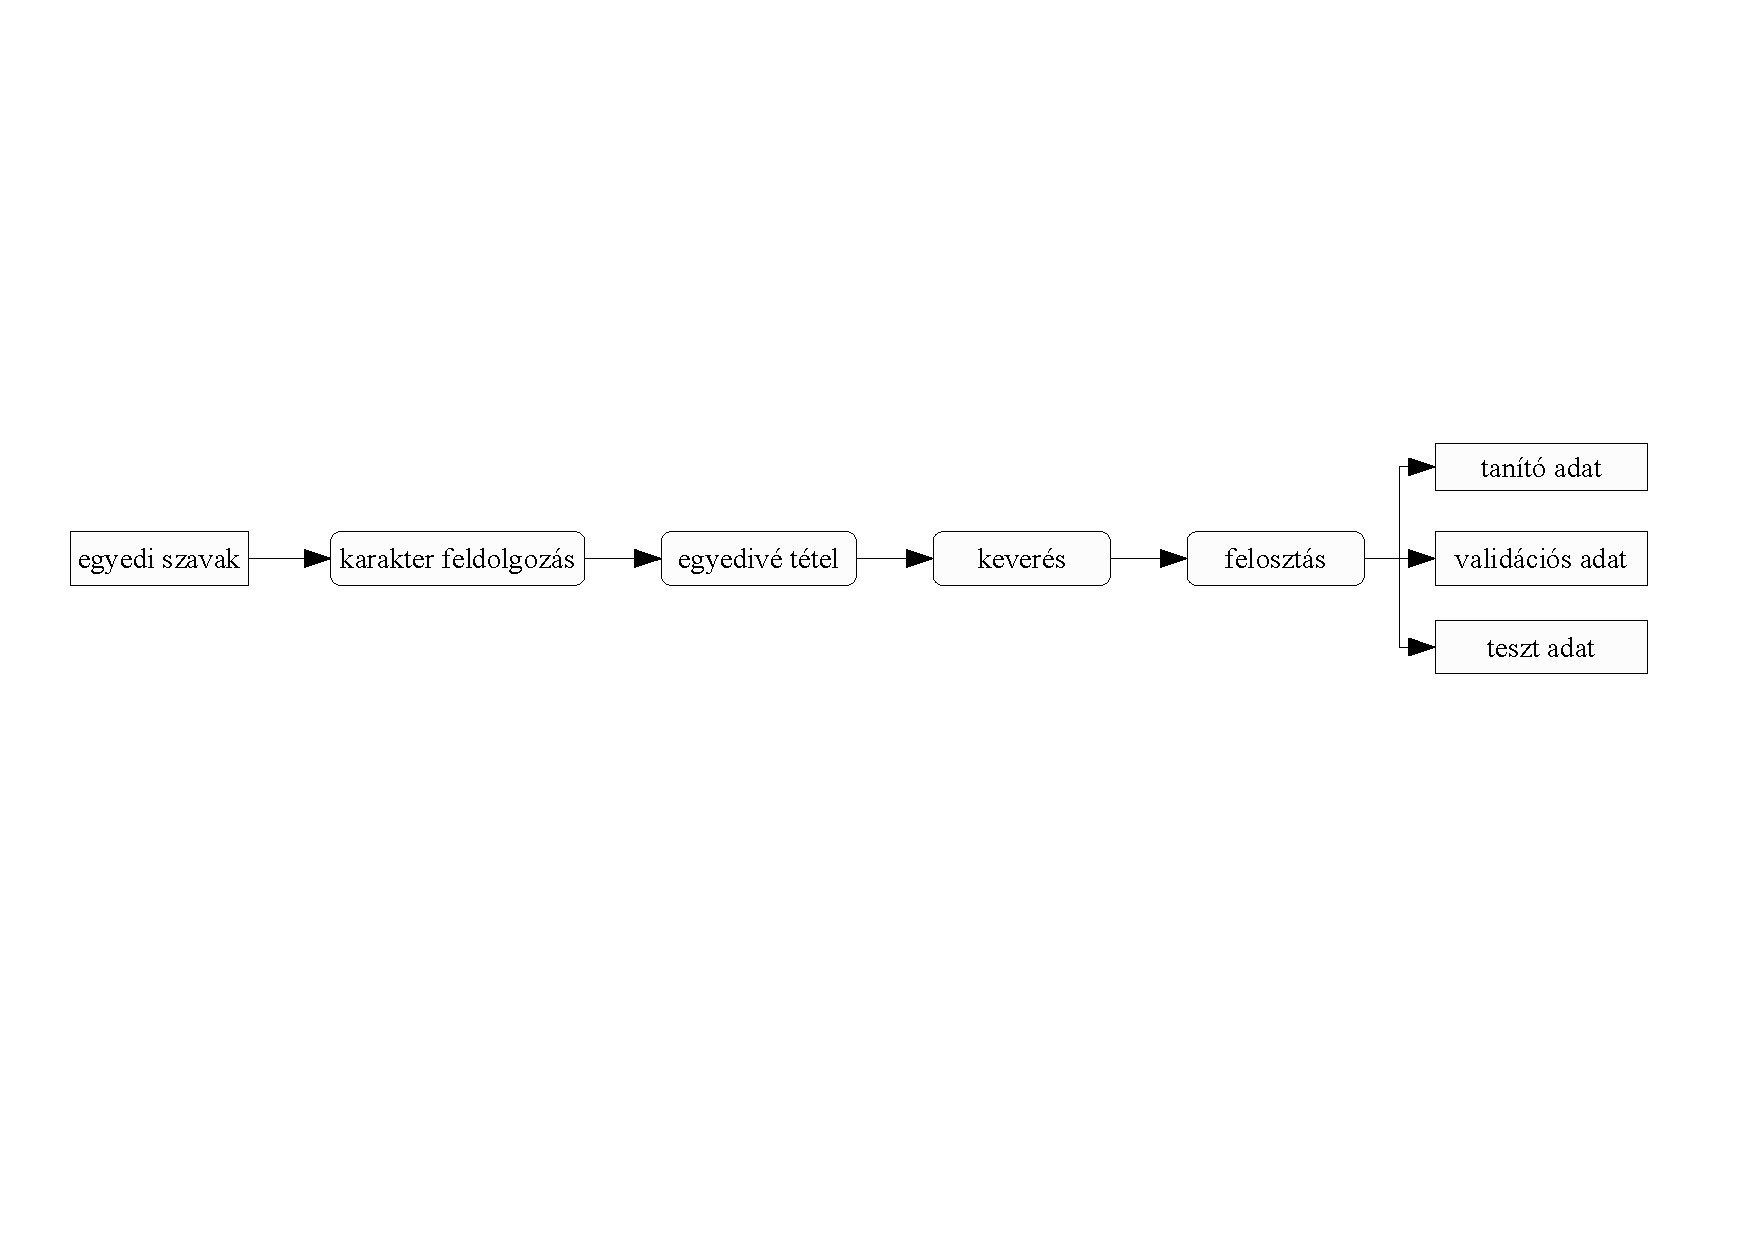
\includegraphics[trim={0 8cm 0 7cm},clip,
	width=\textwidth]{figures/dataflowuchars.pdf}
	\caption{Egyedi adatok}\par\medskip\centering
	\label{fig:dfuchars}
\end{figure}
\section{Eredmények}
Az első tanítások eredményei \tabref{tab:firstlearn}ban láthatóak.

\tabref{tab:optim} a hiperparaméterek optimalizálási eredményeit foglalja össze. Itt a 2-1-2 környezetű karakter-címkézés 2-10 rétegű, rétegenként 10-100 neuronú tanítások közül láthatjuk azokat, amelyeknek validációs hibája megközelíti a 4 százalékot.

\Tabref{tab:winoptim} a karakter címkézéséhez körülötte megvizsgált karakterek számát változtattuk. Jól látható, hogy egy-egy karakter bevétele még jóval kevesebb információt árul el a címkézésről, mint a többi. Hasonlóképp észrevehető, hogy a túl nagy ablak is ront a helyzeten. Ez azért jelenik meg, mivel a nagyobb ablakok bevezetésével egyre ritkábbak lesznek az adott típusú minták előfordulása az adatokban.
\subsection{A táblázatokban használt rövidítések}
\begin{itemize}
	\item Length: \textit{a-1-b} a vizsgált karakter előtt $a$ utána $b$ karaktert veszünk be környezetébe, ami alapján a címkézést végezzük.
	\item Tag: a címkézés BM vagy BMES
	\item NLayer: a háló rejtett rétegeinek száma
	\item NHidden: a rejtett rétegek mérete
	\item Val\_loss: a validációs adatok binary(BM) illetve categorical(BMES) crossentropy hibafüggvénnyel számolt hibája
	\item Test\_w: maximumkiválasztás után hibás eredményt adó teszt adatok száma
	\item Epochs: a tanításhoz szükséges epoch-ok száma. A tanítás végét early stoping módszerrel határoztuk meg.
\end{itemize}
\begin{table}[htp]\centering
	\begin{tabular}{|r|c|c|c|r|r|r|}
		\hline
		No&Tag&Length&Loss&Batch size&Val\_loss&Epochs\\
		\hline\hline
		1&BMES&2-1-0&cat\_cross&512&0.616&483\\ 
		\hline
		2&BM&2-1-0&bin\_cross&1024&0.262&475\\
		\hline
		3&BM&2-1-0&cat\_cross&1024&0.261&543\\
		\hline
		4&BM&2-1-1&bin\_cross&1024&0.063&247\\
		\hline
		5&BM&2-1-2&bin\_cross&1024&0.050&213\\
		\hline
		6&BM&3-1-3&bin\_cross&1024&0.047&223\\
		\hline
		7&BMES&2-1-2&cat\_cross&1024&0.107&389\\
		\hline
		8&BMES&3-1-3&cat\_cross&1024&0.090&769\\
		\hline
	\end{tabular}
	\caption{Előrecsatolt háló tanítása különböző paraméterekkel}
	\label{tab:firstlearn}
\end{table}
\begin{small}
\begin{table}[tp]\centering
	\begin{tabular}{|l|c|r|r|r|r|r|r|}
		\hline
		No&Tag&Length&NLayer&NHidden&Epochs&Val\_loss&Test\_w\\
		\hline\hline
		2.1&BM&2-1-2&2&10&308&0.05025&0.01568\\
		\hline
		2.2&BM&2-1-2&2&20&250&0.04454&0.01352\\
		\hline
		2.3&BM&2-1-2&2&30&189&0.04274&0.01264\\
		\hline
		2.4&BM&2-1-2&2&40&170&0.04151&0.01185\\
		\hline
		2.5&BM&2-1-2&2&50&196&0.04207&0.01129\\
		\hline
		2.6&BM&2-1-2&2&60&167&0.04068&0.01119\\
		\hline
		2.7&BM&2-1-2&2&70&166&0.04155&0.01122\\
		\hline
		2.8&BM&2-1-2&2&80&175&0.03994&0.01073\\
		\hline
		2.9&BM&2-1-2&2&90&179&0.03962&0.01050\\
		\hline
		2.10&BM&2-1-2&2&100&145&0.03911&0.01100\\
		\hline
		3.7&BM&2-1-2&3&70&176&0.04221&0.01155\\
		\hline
		3.8&BM&2-1-2&3&80&161&0.03881&0.01095\\
		\hline
		3.9&BM&2-1-2&3&90&171&0.03872&0.01037\\
		\hline
		3.10&BM&2-1-2&3&100&178&0.03886&0.01062\\
		\hline
		4.7&BM&2-1-2&4&70&208&0.04024&0.01116\\
		\hline
		4.8&BM&2-1-2&4&80&171&0.03995&0.01077\\
		\hline
		4.9&BM&2-1-2&4&90&177&0.03894&0.01077\\
		\hline
		4.10&BM&2-1-2&4&100&177&0.03885&0.01090\\
		\hline
		5.4&BM&2-1-2&5&40&199&0.04423&0.01225\\
		\hline
		5.5&BM&2-1-2&5&50&205&0.03992&0.01136\\
		\hline
		5.6&BM&2-1-2&5&60&220&0.03955&0.01090\\
		\hline
		5.7&BM&2-1-2&5&70&179&0.04013&0.01063\\
		\hline
		\textbf{5.8}&\textbf{BM}&\textbf{2-1-2}&\textbf{5}&\textbf{80}&\textbf{207}&\textbf{0.03937}&\textbf{0.01032}\\
		\hline
		5.9&BM&2-1-2&5&90&218&0.03995&0.01076\\
		\hline
		5.10&BM&2-1-2&5&100&186&0.03927&0.01092\\
		\hline
		6.7&BM&2-1-2&6&70&202&0.04186&0.01149\\
		\hline
		6.8&BM&2-1-2&6&80&218&0.04048&0.01076\\
		\hline
		6.9&BM&2-1-2&6&90&157&0.04715&0.01221\\
		\hline
		6.10&BM&2-1-2&6&100&217&0.03926&0.01072\\
		\hline
		7.7&BM&2-1-2&7&70&254&0.04432&0.01218\\
		\hline
		7.8&BM&2-1-2&7&80&221&0.04335&0.01169\\
		\hline
		7.9&BM&2-1-2&7&90&224&0.03943&0.01046\\
		\hline
		7.10&BM&2-1-2&7&100&210&0.04165&0.01198\\
		\hline
	\end{tabular}

	
	\caption{Hiperparaméter optimalizálás}
	\label{tab:optim}
\end{table}
\end{small}
\begin{small}
\begin{table}[tp]\centering
\begin{tabular}{|l|c|r|r|r|r|r|r|}
			\hline
			No&Tag&Length&NLayer&NHidden&Epochs&Val\_loss&Test\_w\\
\hline\hline
3.6&BM&1-1-1&5&60&303&0.09159&0.03617\\
\hline
3.7&BM&1-1-1&5&70&303&0.09156&0.03634\\
\hline
3.8&BM&1-1-1&5&80&229&0.09155&0.03582\\
\hline
3.9&BM&1-1-1&5&90&252&0.09137&0.03544\\
\hline
3.10&BM&1-1-1&5&100&196&0.09281&0.03595\\
\hline
3.11&BM&1-1-1&5&110&249&0.09129&0.03601\\
\hline
5.6&BM&2-1-2&5&60&222&0.04062&0.01113\\
\hline
5.7&BM&2-1-2&5&70&202&0.03969&0.01069\\
\hline
5.8&BM&2-1-2&5&80&222&0.04209&0.01099\\
\hline
5.9&BM&2-1-2&5&90&214&0.03992&0.01070\\
\hline
5.10&BM&2-1-2&5&100&198&0.03950&0.01049\\
\hline
5.11&BM&2-1-2&5&110&190&0.03995&0.01052\\
\hline
7.6&BM&3-1-3&5&60&133&0.03853&0.00988\\
\hline
7.7&BM&3-1-3&5&70&131&0.04250&0.01096\\
\hline
7.8&BM&3-1-3&5&80&147&0.04433&0.01245\\
\hline
7.9&BM&3-1-3&5&90&149&0.03865&0.00982\\
\hline
7.10&BM&3-1-3&5&100&137&0.03813&0.00972\\
\hline
\textbf{7.11}&BM&\textbf{3-1-3}&\textbf{5}&\textbf{110}&\textbf{136}&\textbf{0.03926}&\textbf{0.00952}\\
\hline
9.6&BM&4-1-4&5&60&121&0.03903&0.01005\\
\hline
9.7&BM&4-1-4&5&70&119&0.04316&0.01143\\
\hline
9.8&BM&4-1-4&5&80&125&0.04126&0.01104\\
\hline
9.9&BM&4-1-4&5&90&118&0.03934&0.01052\\
\hline
9.10&BM&4-1-4&5&100&116&0.03831&0.01072\\
\hline
9.11&BM&4-1-4&5&110&126&0.03967&0.01082\\
\hline
11.6&BM&5-1-5&5&60&112&0.04542&0.01183\\
\hline
11.7&BM&5-1-5&5&70&111&0.04082&0.01087\\
\hline
11.8&BM&5-1-5&5&80&119&0.04566&0.01220\\
\hline
11.9&BM&5-1-5&5&90&99&0.04360&0.01005\\
\hline
11.10&BM&5-1-5&5&100&103&0.04013&0.01035\\
\hline
11.11&BM&5-1-5&5&110&98&0.04117&0.01064\\
\hline
\end{tabular}
\caption{Karakter-környezet ablak méretének optimalizálása}
\label{tab:winoptim}
\end{table}
\end{small}
\newpage
\bibliographystyle{plain}
\bibliography{references}
\addcontentsline{toc}{section}{Hivatkozások}

\end{document}
